\section{Charged Leptons and Neutrons before BBN} 
%%%%%%%%%%%%%%%%%%%%%%%%%%%%%
\subsection{Timeline for charged leptons in the primordial Universe}\label{Electron}
Charged leptons\index{lepton} $\tau^\pm,\mu^\pm,e^\pm$ played significant roles in the dynamics and evolution of the primordial Universe. They were kept in equilibrium via electromagnetic and weak interactions. In this chapter, we examine a dynamical model of the abundance of charged leptons $\mu^\pm$ and $e^\pm$ in the primordial Universe. Of particular interest in this work is the dense electron-positron plasma present during the primordial Universe evolution. We study the damping rate and the magnetization\index{magnetization} process in this dense $e^\pm$ plasma in the primordial Universe.

We comment briefly on the case of $\tau^\pm$-particle which is different as their mass $m_\tau=1776.86$\,MeV is above a threshold allowing the $\tau^\pm$-particle to decay into hadrons in about 2/3 of their decays mediated by the W-gauge boson; the vacuum lifespan for $\tau^\pm$-particle is~\cite{ParticleDataGroup:2022pth}
\begin{align}
&\tau_{\tau}=(290.3\pm0.5)\times10^{-15}\,\mathrm{sec}\,.
\end{align}
$\tau^\pm$-particle disappears at a temperature $T\simeq 75$-$50\MeV$ from the Universe inventory via multi-particle decay processes. This heavy lepton provides an interesting bridge between EM particles, and hadrons, near to QGP hadronization. While the full understanding of $\tau^\pm$-particle dynamics in the primordial Universe would be an interesting topic of future research it is not relevant to the regime we are considering here, with temperature $T<10\MeV$. 

On the other hand, the understanding the $\mu^\pm$-lepton abundance is required for the understanding of several fundamental questions concerning properties of the primordial Universe after emergence of residual baryon asymmetry\index{baryon!asymmetry} below $T=38$\,MeV. Muons play also an important role in the dynamics of the ensuing disappearance of strangeness flavor in the primordial Universe. We recall that the strangeness decay often proceeds into muons, energy thresholds permitting; the charged kaons K$^\pm$ have a 63\% branching into $\mu+\bar \nu_\mu$ decay channel. 

The disappearance of muons\index{muon} has therefore direct impact on strangeness flavor inventory in the primordial Universe. Muons are relatively strongly connected to charged pions through the decay and production reaction 
\begin{align}
&\pi^\pm\leftrightarrow \mu^\pm+\nu_\mu\,.
\end{align}
The decay process is nearly exclusive. The back reaction remains active down to relatively low temperature of a few MeV, as long as muons remain in the primordial Universe thermal population inventory. We conclude that if and when muons fall out of their thermal abundance equilibrium this would directly impact the detailed balance back-reaction processes involving strangeness. 

The lightest charged leptons $e^\pm$ can persist via the reaction $\gamma\gamma\to e^-e^+$ until below $T\simeq 20.3$\,keV any remaining positron rapidly disappears through annihilation, leaving only residual electrons required to maintain the primordial Universe's charge neutrality\index{charge neutrality} considering the baryon\index{baryon} (proton) abundance. The long lasting existence of an electron-positron plasma down to temperature range just above $T=20$\,keV plays a pivotal role in several aspects of the primordial Universe: 

1. The primordial electron-positron plasma\index{plasma!electron-positron} has not received the appropriate attention in the context of precision BBN studies\index{Big-Bang!BBN}. However, the presence of dense $e\bar e$-pair plasma before and during BBN has been recognized already a decade ago by Wang, Bertulani and Balantekin~\cite{Wang:2010px}. The primordial synthesis of light elements is found~\cite{Pitrou:2018cgg} to typically takes place in the temperature range $86\,\mathrm{keV}>T_{BBN}>50\,\mathrm{keV}$. Within this temperature range we show below presence of millions of electron-positron pairs per every charged nucleon and plasma densities which reach millions of times normal atomic particle density~\cite{Yang:2024ret,Grayson:2023flr}. Given that the BBN nucleosynthesis processes occur in an electron-positron-rich plasma environment we explore in this work the effect of modifications in the nuclear repulsive Coulomb potential due to the in plasma screening effects on BBN nuclear reactions~\cite{Grayson:2024okq,Grayson:2024uwg}. 

2. The Universe today is filled with magnetic fields at various scales and strengths, both within galaxies, and in deep extra-galactic space. The origin of these magnetic fields\index{magnetic!fields} is currently unknown. In the primordial Universe, above temperature $T>20$\,keV, we have a dense nonrelativistic $e^\pm$ plasma which could prove to be primordial origin of cosmic magnetism as we describe below~\cite{Steinmetz:2023ucp,Rafelski:2023emw,Steinmetz:2023nsc} and \rsec{sec:mag:universe}. We will show that beyond electric currents the magnetic moments of electrons can contribute to spin based magnetization process.

Understanding the abundances of $\mu^+\mu^-$ and $e^+e^-$-pair plasma provides essential insights into the evolution of the primordial Universe. In the following we discuss the muon density down to their persistence temperature and explore the electron/positron plasma properties, including the QED plasma damping rate and damped dynamic screening in \rsec{section:electron}.

%%%%%%%%%%%%%%%%%%%%%%%%%%%%%%%%%%%%%%%
\para{Muon pairs in the primordial Universe}
Our interest in strangeness flavor freeze-out in the primordial Universe requires the understanding of the abundance of muons in the primordial Universe. The specific question needing an answer is at which temperature muons remain in abundance (chemical) equilibrium established predominantly by electromagnetic and weak interaction processes, allowing diverse detailed-balance back-reactions to influence the primordial strangeness abundance.

In the primordial Universe in the the cosmic plasma muons of mass $m_\mu=105.66$\,MeV can be produced by the following interaction processes~\cite{Yang:2024ret,Rafelski:2021aey}\index{muon!production}
\begin{align} 
\gamma+\gamma&\longrightarrow\mu^++\mu^-,\qquad &e^++e^-\longrightarrow \mu^++\mu^-\;,\\
\pi^-&\longrightarrow\mu^-+\bar{\nu}_\mu,\qquad &\pi^+ \longrightarrow\mu^++\nu_\mu\;.
\end{align}
The back reactions for all above processes are in detailed balance, provided all particles shown on the right hand side (RHS) exist in chemical abundance equilibrium in the primordial Universe. We recall the empty space (no plasma) at rest lifetime of charged pions $\tau_\pi=2.6033\times 10^{-8}$\,s. We note that neutral pions decay much faster $\tau_{\pi^0}=8.43\times 10^{-17}$\,s.\index{pion!decay}

Any of the produced muons can decay via the well known reactions
\begin{equation}
\mu^-\rightarrow\nu_\mu+e^-+\bar{\nu}_e,\qquad \mu^+\rightarrow\bar{\nu}_\mu+e^++\nu_e\,,
\end{equation} 
with the empty space (no plasma) at rest lifetime $\tau_{\mu}=2.197 \times 10^{-6}\,\mathrm{s}$. 
 
The temperature range of our interests is the Universe when $m_\mu\gg T$. In this case the Boltzmann approximation\index{Boltzmann!approximation} is appropriate for studying massive particles such as muons and pions. The thermal decay rate per volume and time for muons $\mu^\pm$ (and pions $\pi^\pm$) in the Boltzmann limit are given by~\cite{Kuznetsova:2010pi}:\index{muon!decay rate}
\begin{align}
&R_\mu=\frac{g_\mu}{2\pi^2}\left(\frac{T^3}{\tau_\mu}\right)\left(\frac{m_\mu}{T}\right)^2K_1(m_\mu/T)\;,\\
&R_\pi=\frac{g_\pi}{2\pi^2}\left(\frac{T^3}{\tau_\pi}\right)\left(\frac{m_\pi}{T}\right)^2K_1(m_\pi/T)\;, 
\end{align}
where the lifespan of $\mu^\pm$ and $\pi^\pm$ in the vacuum were given above. This rate accounts for both the density of particles in chemical abundance equilibrium and the effect of time dilation present when particles are in thermal motion with respect to observer at rest in the local reference frame. The quantum effects of Fermi blocking or boson stimulated emission have been neglected using Boltzmann statistics.

%%%%%%%%%%%%%%%%%%%%%%%%%%%%%%%%%
\para{Muon production processes}
The thermal averaged reaction rate per volume for the reaction $a\overline{a}\rightarrow b\overline{b}$ in Boltzmann approximation is given by~\cite{Letessier:2002ony}\index{muon!production rate}
\begin{align}\label{pairR}
R_{a\overline{a}\rightarrow b\overline{b}}=\frac{g_ag_{\overline{a}}}{1+I}\frac{T}{32\pi^4}\int_{s_{th}}^\infty ds\frac{s(s-4m^2_a)}{\sqrt{s}}\sigma_{a\overline{a}\rightarrow b\overline{b}}~K_1(\sqrt{s}/T),
\end{align}
where $s_{th}$ is the threshold energy for the reaction, $\sigma_{a\overline{a}\rightarrow b\overline{b}}$ is the cross-section for the given reaction, and $K_1$ is the modified
Bessel\index{Bessel function} function of integer order ``$1$". We introduce the factor $1/1+I$ to avoid the double counting of indistinguishable pairs of particles; we have $I=1$ for an identical pair and $I=0$ for a distinguishable pair.

The leading order invariant matrix elements for the reactions $e^++e^-\to\mu^++\mu^-$ and $\gamma+\gamma\to\mu^++\mu^-$, are introduced in this work by~\cite{Kuznetsova:2008jt}
\begin{align}\label{Mee}
|M_{e\bar e\to\mu\bar\mu}|^2=&32\pi^2\alpha^2\frac{(m_\mu^2-t)^2+(m_\mu^2-u)^2+2m_\mu^2s}{s^2},\quad m_\mu\gg m_e\;,\\[0.2cm]
\label{Mgg}
|M_{\gamma\gamma\to\mu\bar\mu}|^2=&32\pi^2\alpha^2\bigg[\left(\frac{m_\mu^2-u}{m_\mu^2-t}+\frac{m_\mu^2-t}{m_\mu^2-u}\right)+4\left(\frac{m_\mu^2}{m_\mu^2-t}+\frac{m_\mu^2}{m^2_\mu-u}\right)\\[0.1cm] \nonumber
&\hspace{1cm}-4\left(\frac{m_\mu^2}{m^2_\mu-t}+\frac{m^2_\mu}{m^2_\mu-u}\right)^2\bigg]\;,
\end{align}
 where $s, t, u$ are the Mandelstam variables\index{Mandelstam variables}. The cross-section required in \req{pairR} can be obtained by integrating the matrix elements \req{Mee} and \req{Mgg} over the Mandelstam variable $t$~\cite{Kuznetsova:2010pi}. We have
\begin{align}
\sigma_{e\bar e\to\mu\bar\mu} 
&=\frac{64\pi\alpha^2}{48\pi}\left(\frac{1+2m^2_\mu/s}{s-4m_e^2}\right)\beta\,,\qquad 
\beta =\sqrt{1-\frac{4m^2_\mu}{s}}\, ,\\
%\sqrt{1-\frac{4m^2_\mu}{s}},\\
\sigma_{\gamma\gamma\to\mu\bar\mu}
 &=\frac{\pi}{2}\left(\frac{\alpha}{m_\mu}\right)^2(1-\beta^2)\left[(3-\beta^4)\ln\frac{1+\beta}{1-\beta}-2\beta(2-\beta^2)\right] \,.
\end{align}
Substituting the cross-sections into \req{pairR} we obtain the production rates for $e\bar e\to\mu\bar\mu$ and $\gamma\gamma\to\mu\bar\mu$, respectively.

As the temperature decreases in the expanding Universe, the initially dominant production rates ($e\bar e,\gamma\gamma\to\mu\bar\mu$) decrease with decreasing temperature, and eventually cross the $\mu^\pm$ decay rates. The muon abundance disappears as soon as any known decay rate is faster than the fastest production rate. In \rf{MuonRatenew:fig} we show the invariant thermal reaction rates per volume and time for rates of relevance, as a function of temperature $T$. It is important to first note that the pion decay rate (short-long dashed, black) is smaller compared to the other rates in the domain of temperatures we are interested. The weak decay rate of the muon is shown by dotted line (green)\index{muon!decay}. The dominant reactions for $\mu^\pm$ production are ${\gamma+\gamma\to\mu^++\mu^-}$ (dashed, blue) and $e^++e^-\to\mu^++\mu^-$ (dashed, red), the solid line (violet) shows the sum of both rates. 

 
%%%%%%%%%%%%%%%%%%%%%%%%%%
\begin{figure}
\centerline{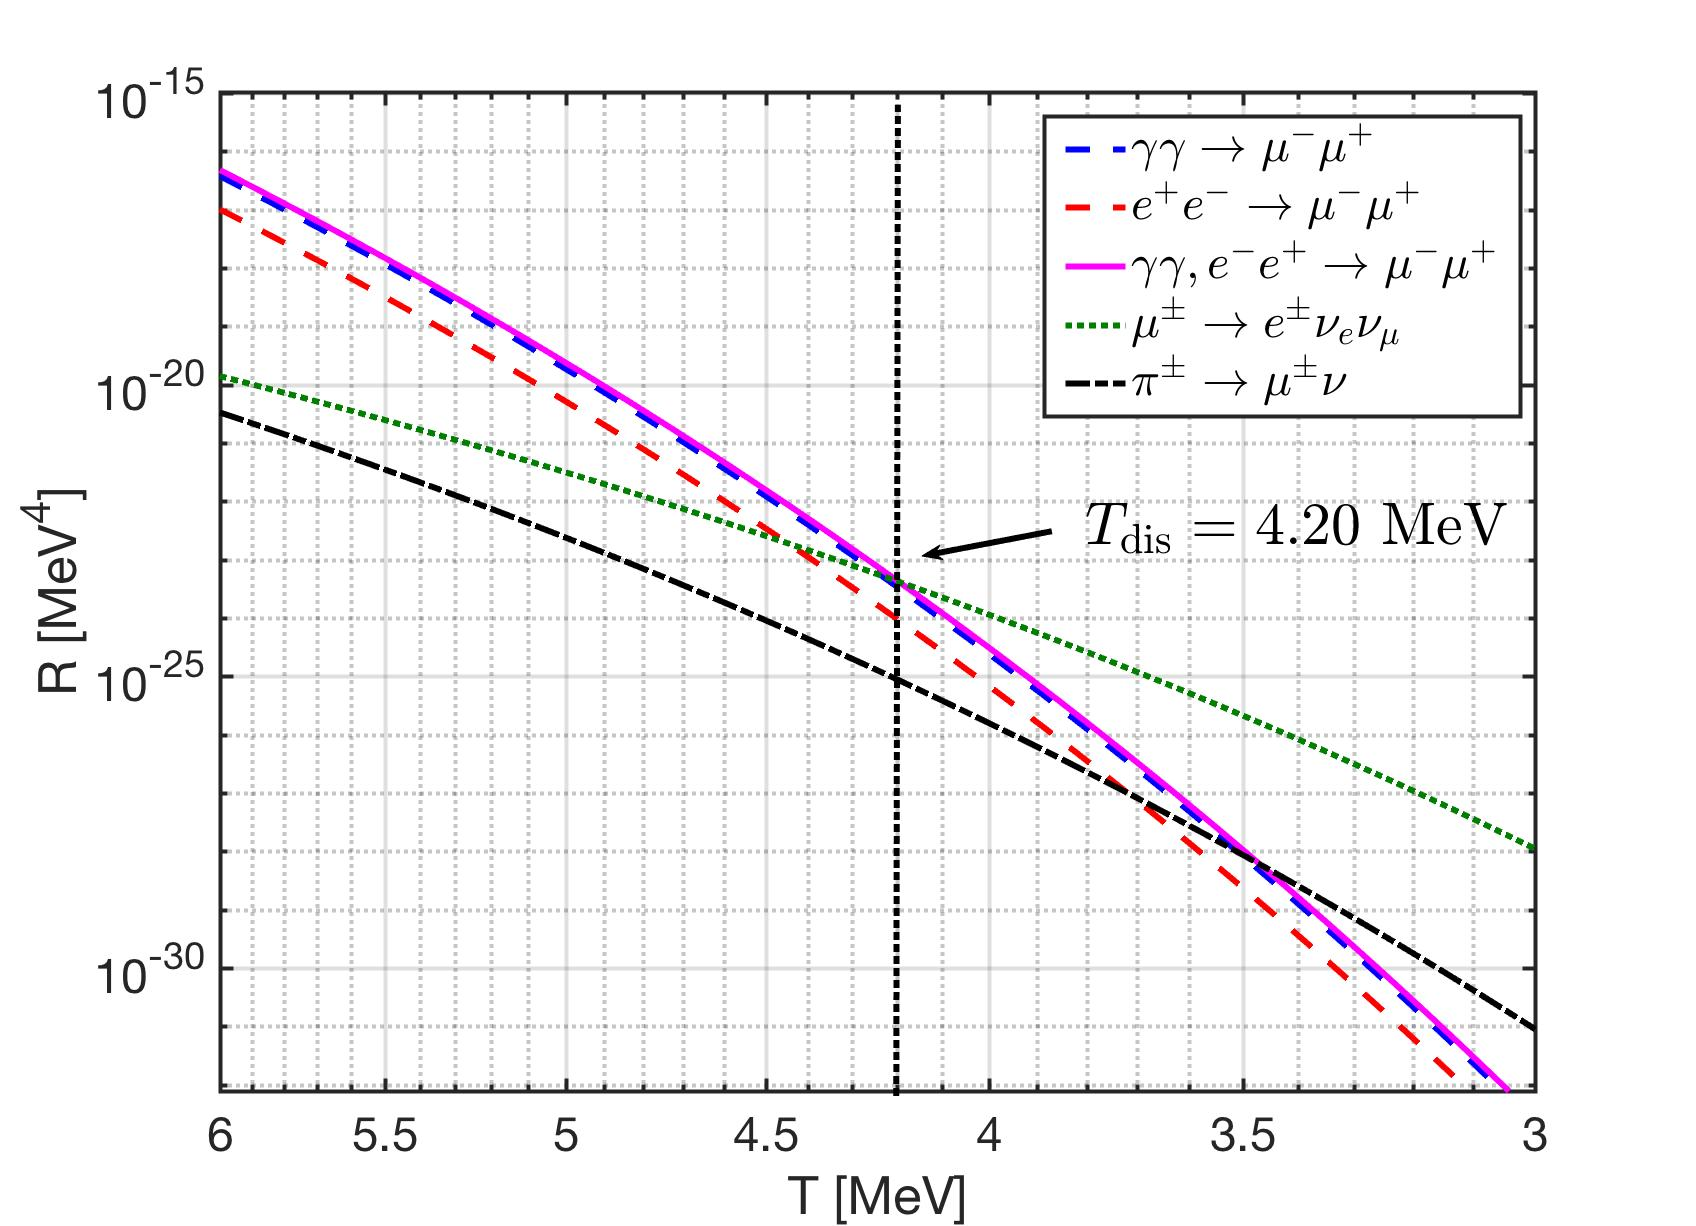
\includegraphics[width=0.8\linewidth]{./plots/MuonRate_new2.jpg}}
\caption{The thermal reaction rate per time and volume for different muon reactions as a function of temperature. See text.\cccite{Rafelski:2023emw}. \radapt{Yang:2024ret,Rafelski:2021aey}}
\label{MuonRatenew:fig} 
\end{figure}
%%%%%%%%%%%%%%%%%%%%%%%%%%%%%%

The total $\mu^\pm$ production rate crosses the decay rate at temperature $T_{dissapear}\approx 4.195$\,MeV. Due to the relatively slow expansion of the Universe, the disappearance of muons\index{muon!disappearance} is sudden, and the abundance of muons vanishes as soon as a fast microscopic decay rate surpasses the total production rate. We see that irrespective of charged pion abundance, muons persist until the Universe cools below the temperature $T_\mathrm{disappear}=4.195$\,MeV, below that temperature the dominant reaction is the muon decay.


%%%%%%%%%%%%%%%%%%%%%%%%%%%%%%%%%
\para{Comparison of muon and baryon abundance}
It is of interest to explore and to compare the muon inventory in the Universe with the baryon number inventory. Considering the number density for nonrelativistic $\mu^\pm$ in the Boltzmann approximation, we obtain
\begin{align}\label{nmupm}
n_{\mu^\pm}=\frac{g_{\mu^\pm}}{2\pi^2}T^3\left(\frac{m_\mu}{T}\right)^2 K_2(m_\mu/T)=g_{\mu^\pm}\left(\frac{m_\mu T}{2\pi}\right)^{3/2}e^{-{m_\mu}/{T}}\;. 
\end{align}
The ration of the number density between $n_{\mu^\pm}$ and baryons\index{baryon} $n_B$ can be written as follows
\begin{align}
\frac{n_{\mu^\pm}}{n_\mathrm{B}}=\frac{n_{\mu^\pm}}{\sigma}\frac{\sigma}{n_\mathrm{B}}=
\frac{n_{\mu^\pm}}{\sigma}\left[\frac{\sigma}{n_\mathrm{B}}\right]_{t_0},
\end{align}
where we assume that $\sigma/n_\mathrm{B}$ the ratio of entropy to baryon number remains constant and $t_0$ represent present day value. The present value is given by $(n_B/\sigma)_{t_0}\approx8.69\times10^{-11}$\index{baryon!entropy ratio}. We recall, see \rf{EntropyDOF:Fig}, that the entropy density\index{entropy!density} $\sigma$ can be characterized introducing $g^s_\ast$, the total number of \lq entropic\rq\ degrees of freedom, see \req{eq:entg}. For temperature $10\,\mathrm{MeV} >T>3 $\,MeV, the massless photons, nearly relativistic electrons and positrons, and practically massless neutrinos contribute to the count of degrees of freedom $g^s_\ast$. In this case, the number density between $n_{\mu^\pm}$ and baryon $n_B$ in the temperature interval we consider $10\,\mathrm{MeV} >T>3 $\,MeV is given by
\begin{align}\label{nmuperbF} 
\frac{n_{\mu^\pm}}{n_\mathrm{B}}=\frac{45}{2\pi^2}\frac{g_{\mu^\pm}}{g^s_\ast}\left(\frac{m_\mu}{2\pi T}\right)^{3/2}e^{-{m_\mu}/{T}}\;\left(\frac{\sigma}{n_\mathrm{B}}\right)_{\!t_0}.
\end{align}

In \rf{fig:DensityRatio} we show the muon to baryon density ratio \req{nmuperbF} as a function of $T$\index{muon!to baryon ratio}. We see that the very small muon pair abundance at $T=10$\,MeV exceeds that of residual baryons by a large factor 500,000, while at muon disappearance temperature $n_{\mu^\pm}/n_\mathrm{B}(T_\mathrm{disappear})\approx0.911$. The number density $n_{\mu^\pm}$ and $n_\mathrm{B}$ abundances are equal at the temperature $T_\mathrm{equal}\approx4.212\,\mathrm{MeV} > T_\mathrm{disappear}$. 

%%%%%%%%%%%%%%%%%%%%%%%%%%%%%%%%%%%%%
\begin{figure}
\centerline{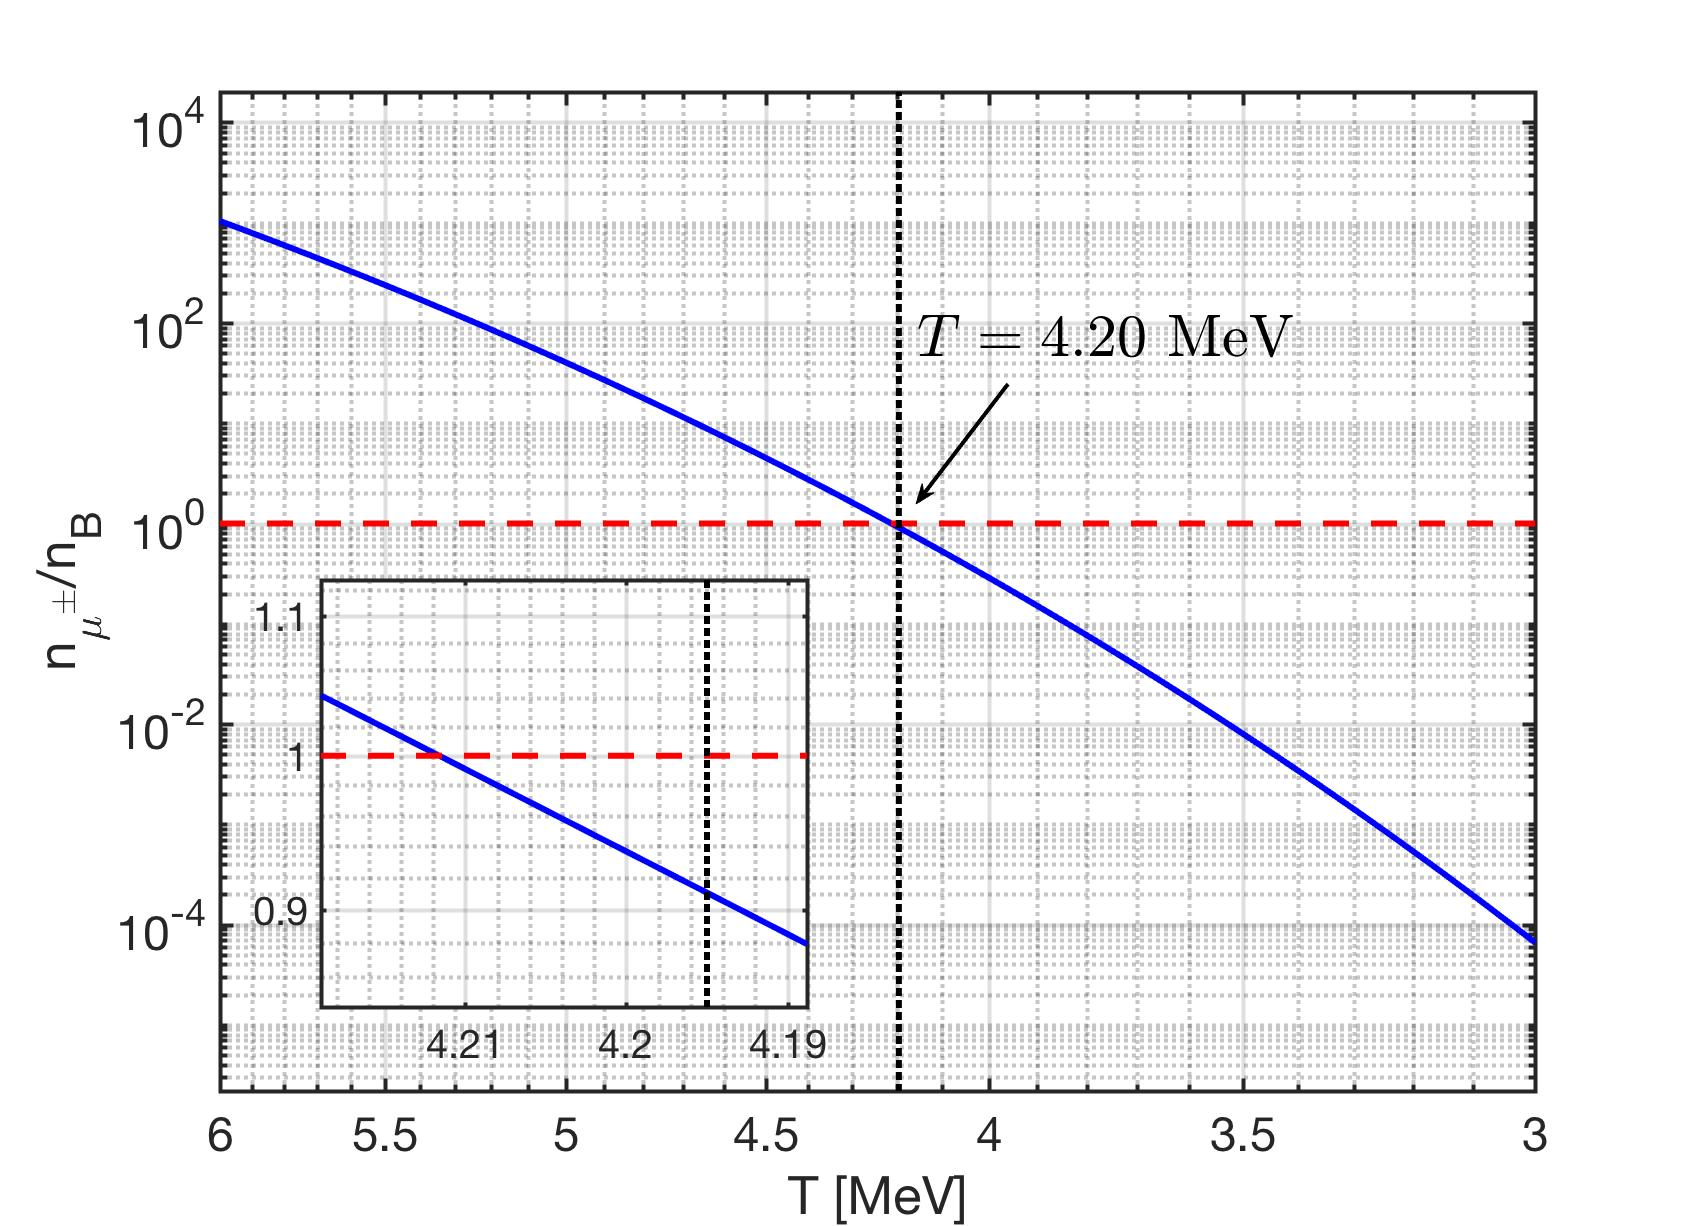
\includegraphics[width=0.8\linewidth]{./plots/DensityRatio_new2.jpg}}
\caption{The density ratio between $\mu^\pm$ and baryons as a function of temperature. The density ratio at muon disappearance temperature is $n_{\mu^\pm}/n_\mathrm{B}(T_\mathrm{disappear})\approx0.911$, and around the temperature $T\approx4.212$\,MeV the computed density ratio $n_{\mu^\pm}/n_\mathrm{B}\approx1$. \cccite{Rafelski:2023emw}. \radapt{Yang:2024ret,Rafelski:2021aey}}
\label{fig:DensityRatio}
\end{figure}
%%%%%%%%%%%%%%%%%%%%%%%%

\index{muon!baryon ratio}
The primary insight is that aside of protons, neutrons and other nonrelativistic particles, both positively and negatively charged muons $\mu^\pm$ are present in thermal equilibrium and in non-negligible abundance exceeding baryon abundance down to $T>T_\mathrm{dissapear}\approx 4.195$\,MeV. This coincidence, muon and baryon abundance being practically equal at temperature of muon disappearance, surprised us. We do not know if there is a physics content in this observation. 

%%%%%%%%%%%%%%%%%%%%%%%%%%%%
\subsection{Cosmic electron-positron plasma and BBN}
\label{section:electron}
Following on the neutrino freeze-out at $T\approx 2$\,MeV, the Universe is dominated by the electron-positron-photon QED plasma. In this section, we derive the electron-positron density and chemical potential\index{chemical potential!charge neutrality} required for local charge neutrality\index{Universe!charge neutrality} of the Universe to show that during the normal BBN\index{Big-Bang!BBN} temperature range $86.7\,\mathrm{keV}>\mathrm{T_{BBN}}>50\,\mathrm{keV}$~\cite{Pitrou:2018cgg} the Universe was filled with a dense electron-positron pair-plasma dotted with a dispersed baryonic matter dust. 

We examine the microscope collision properties of the electron-positron plasma in the primordial Universe allowing us to use appropriately generalized methods of plasma physics in a study of the role of the $e^+e^-$ plasma in the primordial Universe. The time scale of Universe expansion $H^{-1}$ is orders of magnitude larger than the microscopic reaction time scales of interest for all processes we consider, the dynamical processes we consider are thus occurring in expanding, but stationary Universe\index{Universe!stationray}.

%%%%%%%%%%%%%%%%%%%%%%%%%%%%%%%%%%%%%%%%%%%%
\para{Electron chemical potential and number density}
We obtain the dependence of electron chemical potential\index{chemical potential!electron}, and hence $e^+e^-$ density, as a function of the photon background temperature $T$ by employing the following physical principles
\begin{enumerate}
\item Charge neutrality of the Universe:
\begin{align}\label{neutrality}
n_{e^-}-n_{{e^+}}=n_p-n_{\overline{p}}\approx\,n_p,
\end{align}
where $n_\ell$ denotes the number density of particle type $\ell$.
\item Neutrinos decouple (freeze-out) at a temperature $T_f\simeq 2$\,MeV, after which they free stream through the Universe with an effective temperature~\cite{Birrell:2012gg}
\begin{align}
 T_\nu(t)=T_f\,\frac{a(t_f)}{a(t)},
\end{align}
where $a(t)$ is the Friedmann-Lema\^{i}tre-Robertson-Walker (FLRW)\index{cosmology!FLRW} Universe scale factor (see cosmology primer \rsec{sec:flrw}) which is a function of cosmic time $t$, and $t_f$ represents the cosmic time when neutrino freezes out.
\item The total comoving entropy is conserved. At $T\leq T_f$, the dominant contributors to entropy are photons, $e^+e^-$, and neutrinos. In addition, after neutrino freeze out, neutrino comoving entropy is independently conserved~\cite{Birrell:2012gg}. This implies that the combined comoving entropy in $e^+e^-\gamma$ is also conserved for $T\leq T_f$.\index{entropy!conservation}
\end{enumerate} 
Motivated by the fact that comoving entropy in $\gamma$, $e^+e^-$ is conserved after neutrino freeze-out, we rewrite the charge neutrality condition, \req{neutrality}, in the form
\begin{align}\label{charge_neutral_cond2}
n_{e^-}-n_{{e^+}}=X_p\frac{n_B}{\sigma_{\gamma,e^\pm}} \sigma_{\gamma,e^\pm},\qquad X_p\equiv\frac{n_p}{n_B},
\end{align}
where $n_B$ is the number density of baryons, $s_{\gamma,e^\pm}$ is the combined entropy density\index{entropy!density} in photons, electrons, and positrons. During the Universe expansion, the comoving entropy and baryon number are conserved quantities; hence the ratio $n_B/\sigma_{\gamma,e^\pm}$ is conserved. We have
\begin{align}
\frac{n_B}{\sigma_{\gamma,e^\pm,}}=\left(\frac{n_B}{\sigma_{\gamma,e^\pm}}\right)_{t_0}\!\!\!\!=\left(\frac{n_B}{\sigma_{\gamma}}\right)_{t_0}\!\!\!\!=\left(\frac{n_B}{n_\gamma}\right)_{t_0}\left(\frac{n_\gamma}{s_{\gamma}}\right)_{t_0},
\end{align}
where the subscript $t_0$ denotes the present day value, and the second equality is obtained by observing that the present day $e^+e^-$-entropy density is negligible compared to the photon entropy density. We can evaluate the ratio introducing the present day baryon-to-photon ratio: $B/N_\gamma =n_B/n_\gamma= 0.605\times10^{-9}$ as obtained from the Cosmic Microwave Background (CMB)~\cite{ParticleDataGroup:2022pth}\index{CMB}, and the entropy per particle for a massless boson: $(s/n)_{\mathrm{boson}}\approx 3.602$.

The total entropy density of photons, electrons, and positrons can be written as
\begin{align}\label{entropy_per_baryon}
\sigma_{\gamma,e^\pm}=\frac{2\pi^2}{45}g_\gamma\,T^3+\frac{\rho_{e^\pm}+P_{e^\pm}}{T}-\frac{\mu_e}{T}(n_{e^-}-n_{{e^+}}),
 \end{align}
where $ \rho_{e^\pm}=\rho_{e^-}+\rho_{e^+}$ and $P_{e^\pm}=P_{e^-}+P_{{e^+}}$ are the total energy density and pressure of electrons and positron respectively.

By incorporating \req{charge_neutral_cond2} and \req{entropy_per_baryon}, the charge neutrality condition can be expressed as
\begin{align}\label{charge_neutral_cond3}
 &\left[1+X_p\left(\frac{n_B}{n_\gamma}\right)_{\!t_0}\!\!\left(\frac{n_\gamma}{\sigma_{\gamma}}\right)_{\!t_0}\!\!\frac{\mu_e}{T}\right]\frac{n_{e^-}-n_{{e^+}}}{T^3}=X_p\left(\frac{n_B}{n_\gamma}\right)_{\!t_0}\!\!\left(\frac{n_\gamma}{\sigma_{\gamma}}\right)_{\!t_0}\!\!\left(\frac{2\pi^2}{45}g_\gamma+\frac{\rho_{e^\pm}+P_{e^\pm}}{T^4}\right).
\end{align}

Using the Fermi distribution, the number density of electrons over positrons in the primordial Universe is given by
\begin{align}\label{ee_density}
n_{e^-}-n_{{e^+}}&=\frac{g_e}{2\pi^2}\left[\int_0^\infty\frac{p^2dp}{\exp{\left((E-\mu_e)\right)/T}+1}\right.\left.-\int_0^\infty\frac{p^2dp}{\exp{\left((E+\mu_e)/T\right)}+1}\right]\notag\\
&=\frac{g_e}{2\pi^2}\,{T^3}\,\tanh(b_e)M_e^3\int_{1}^\infty \!\!\!\!\frac{ \zeta \sqrt{\zeta^2-1} d\zeta}{1+\cosh(M_e\zeta)/\cosh(b_e)},
\end{align}
where we have introduced the dimensionless variables as follows: 
\begin{align}\label{Variables}
\zeta=\frac{E}{m_e},\qquad M_e=\frac{m_e}{T},\qquad b_e=\frac{\mu_e}{T}.
\end{align}
Substituting \req{ee_density} into \req{charge_neutral_cond3} and giving the value of $X_p$, then the charge neutrality condition can be solved to determine $\mu_e/T$ as a function of $M_e$ and $T$. 


In \rf{BBN:Electron} (left axis), we show (left axis, brown line) the electron chemical potential\index{chemical potential} as a function of temperature we obtain solving \req{charge_neutral_cond3} numerically employing the following parameters: proton concentration $X_p=0.878$ as derived from observation~\cite{ParticleDataGroup:2022pth} and $n_B/n_\gamma=6.05\times10^{-10}$ from CMB. We can see the value of chemical potential is comparatively small $\mu_e/T\approx10^{-6}\sim10^{-7}$ during the BBN epoch temperature range, implying a very small asymmetry in the number of electrons and positrons in plasma is needed to neutralize proton charge. 

%%%%%%%%%%%%%%%%%%%%%%%%%%%%%%%%%%%%%%%%%%%%%%%%%%%%%%
\begin{figure}
\centerline{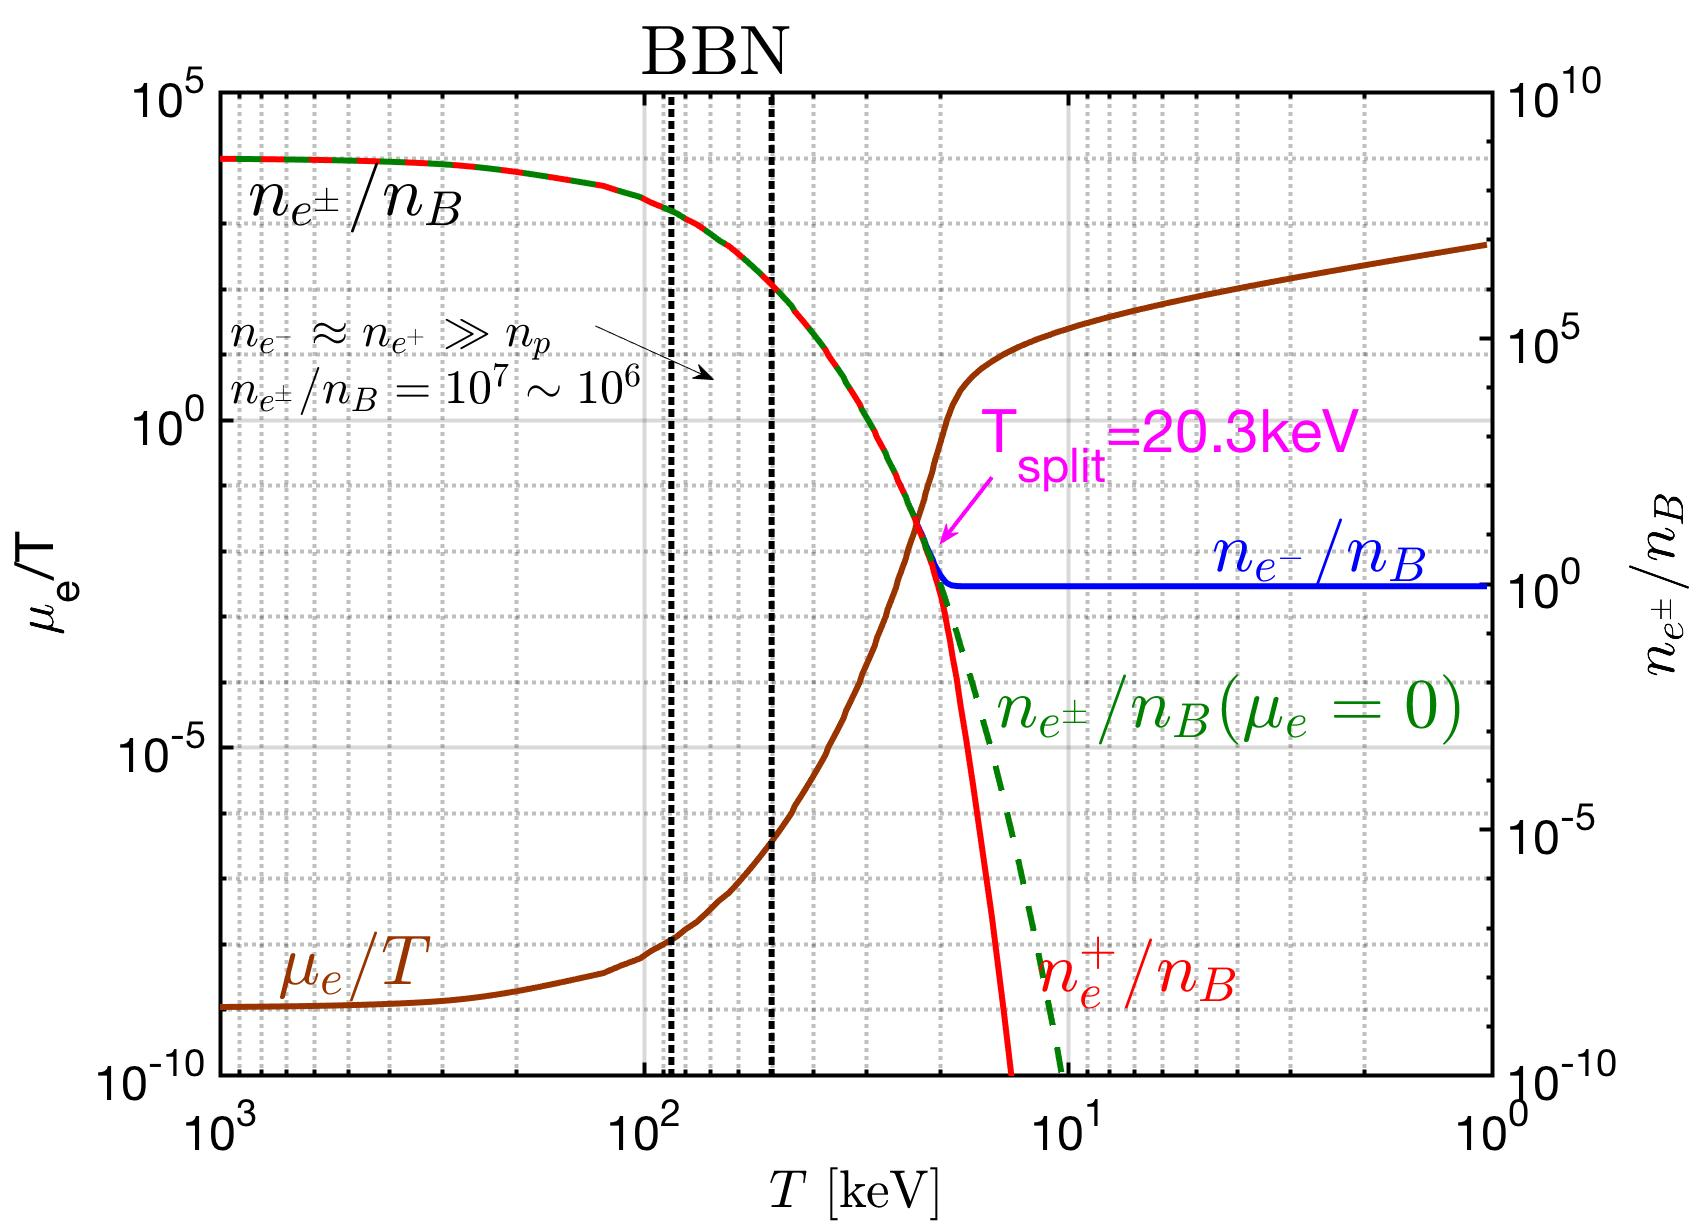
\includegraphics[width=0.8\linewidth]{plots/May152023_EPDensity_Chemical}}
\caption{Left axis: The chemical potential of electrons $\mu_e/T$ as a function of temperature (solid (brown) line). Right axis: the ratio of electron (positron) number density to baryon density as a function of temperature. The solid blue line is the electron density, the red line is the positron density, and the green dashed line is obtained setting for comparison $\mu_e=0$. The vertical black dotted lines are bounds of BBN epoch. \cccite{Grayson:2023flr}. \radapt{Yang:2024ret}}
\label{BBN:Electron}
\end{figure}
%%%%%%%%%%%%%%%%%%%%%%%%%%%%%%%%%

The ratio of electron (positron) number density to baryon density,right axis in \rf{BBN:Electron}, shows that the Universe was filled with an electron-positron rich plasma during the BBN temperature range epoch in the (approximate) temperature range $86\,\mathrm{keV}>\mathrm{T_{BBN}}>50\,\mathrm{keV}$. When the temperature is \eg\ around $T=70\,\mathrm{keV}$, the density of electrons and positrons is comparatively large $n_{e^\pm}\approx10^7\,n_B$. At $90$\,keV, the electron and positron density is near the solar core density, compare Fig.~19 in Ref.~\cite{Rafelski:2023emw}. Near and below the temperature $T=20.3\,\mathrm{keV}$, the positron density decreases rapidly, transforming the pair-plasma into an electron-baryon plasma.

%%%%%%%%%%%%%%%%%%%%%%%%%%%%%%%%%%%%%%%%%%%%
\para{QED plasma damping rate}
\index{plasma!QED damping}
The reactions of interest for the evaluation of the QED plasma damping are the (inverse) Compton scattering\index{Compton scattering}, the M{\o}ller\index{M{\o}ller scattering} scattering, and the Bhabha\index{Bhabha scattering} scattering, respectively
\begin{align}
e^\pm+\gamma\longrightarrow e^\pm+\gamma,\qquad e^\pm+e^\pm\longrightarrow e^\pm+e^\pm,\qquad e^\pm+e^\mp\longrightarrow e^\pm+e^\mp.
\end{align}
The general formula for thermal reaction rate per volume is discussed in~\cite{Letessier:2002ony} (Eq.(17.16), Chapter 17). For inverse Compton scattering we have
\begin{align}
R_{e^{\pm}\gamma}=\frac{g_eg_\gamma}{16\left(2\pi\right)^5}T\int_{m_e^2}^\infty\!\!\!\!ds\frac{K_1(\sqrt{s}/T)}{\sqrt{s}}\int^0_{-(s-m_e^2)^2/s}\!\!\!\!\!\!dt\, |M_{e^{\pm}\gamma}|^2,
\end{align} 
and for M{\o}ller and Bhabha reactions we have
\begin{align}
&R_{e^\pm e^\pm}=\frac{g_eg_e}{16\left(2\pi\right)^5}T\!\!\int_{4m_e^2}^\infty\!\!\!\!ds\frac{K_1(\sqrt{s}/T)}{\sqrt{s}}\int^0_{-(s-4m_e^2)}\!\!\!\!\!\!dt\,|M_{e^\pm e^\pm}|^2,\\[0.3cm]
&R_{e^\pm e^\mp}=\frac{g_eg_e}{16\left(2\pi\right)^5}T\!\!\int_{4m_e^2}^\infty\!\!\!\!ds\frac{K_1(\sqrt{s}/T)}{\sqrt{s}}\int^0_{-(s-4m_e^2)}\!\!\!\!\!\!dt\,|M_{e^\pm e^\mp}|^2,
\end{align}
where $g_i$ is the degeneracy of particle $i$, $|M|^2$ is the matrix element for a given reaction, $K_1$ is the Bessel\index{Bessel function} function of order $1$, and $s,t,u$ are Mandelstam variables\index{Mandelstam variables}. The leading order matrix element associated with inverse Compton scattering can be expressed in the Mandelstam variables~\cite{Kuznetsova:2011wt,Kuznetsova:2009bq} we have\index{Compton scattering}
\begin{align}
|M_{e^\pm\gamma}|^2\!=32 \pi^2\alpha^2\bigg[&4\left(\frac{m_e^2}{m_e^2-s}+\frac{m_e^2}{m_e^2-u}\right)^2
%\notag\\&\qquad\qquad
-\frac{4m_e^2}{m_e^2-s}-\frac{4m_e^2}{m_e^2-u} -
 \frac{m_e^2-u}{m_e^2-s} -\frac{m_e^2-s}{m_e^2-u}\bigg],
\end{align}
and for M{\o}ller\index{M{\o}ller scattering} and Bhabha scattering we have \index{Bhabha scattering}
\begin{align}
|M_{e^{\pm}e^{\pm}}|^{2}\!=64\pi^{2}\alpha^{2}\bigg[&
\frac{s^{2}+u^{2}+8m_e^{2}(t-m_e^{2})}{2(t-m^2_{\gamma})^{2}}
%\notag\\&\quad
+\frac{{s^{2}+t^{2}}+8m_e^{2}
(u-m_e^{2})}{2(u-m_{\gamma}^2)^{2}} + \frac{\left( {s}-2m_e^{2}\right)\left({s}-6m_e^{2}\right)}
{(t-m_{\gamma}^2)(u-m_{\gamma}^2)} \bigg],
\end{align}
and
\begin{align}
|M_{e^\pm e^\mp}|^{2}=64\pi^{2}\alpha^{2}
\bigg[&\frac{s^{2}+u^{2}+8m_e^{2}(t-m_e^{2})}{2(t-m^2_{\gamma})^{2}}
%\notag\\&\quad
+\frac{u^{2}+t^{2}+8m_e^{2}
(s-m_e^{2})}{2(s-m^2_{\gamma})^{2}} + \frac{\left({u}-2m_e^{2}\right)\left({u}-6m_e^{2}\right)}
 {(t-m^2_{\gamma})(s-m^2_{\gamma})} \bigg],
\label{M_fi_b}
\end{align}
where we introduce the photon mass $m_\gamma$ to account the plasma effect and avoid singularity in reaction matrix elements. 

The photon mass $m_\gamma$ in plasma is equal to the plasma frequency $\omega_p$, where we have~\cite{Kislinger:1975uy}\index{photon!plasma mass}
\begin{align}
m^2_\gamma=\omega^2_{p}=8\pi\alpha\int\frac{d^3p_e}{(2\pi)^3}\left(1-\frac{p_e^2}{3E_e^2}\right)\frac{f_e+f_{\bar e}}{E_e},
\end{align}
where $E_e=\sqrt{p_e^2+m^2_e}$. In the BBN temperature range $86\,\mathrm{keV}>T_{BBN}>50\,\mathrm{keV}$ we have $m_e\gg T$ and considering the nonrelativistic limit for electron-positron plasma, we obtain
\begin{align}
m^2_\gamma=\frac{4\pi\alpha}{2m_e}\left(\frac{2m_eT}{\pi}\right)^{3/2}e^{-m_e/T}\cosh\left(\frac{\mu_e}{T}\right).
\end{align}
In the BBN temperature range, we have $\mu_e/T\ll1$, which implies the equal number of electrons and positrons in plasma.

To discuss the collisions plasma by the linear response theory, it is convenient to define the average relaxation rate for the electron-positron plasma as follows:\index{plasma!electron-positron}
\begin{align}\label{Kappa}
\kappa=\frac{R_{e^\pm e^\pm}+R_{e^\pm e^\mp}+R_{e^\pm\gamma}}{\sqrt{n_{e^-}n_{e^+}}}\approx\frac{R_{e^\pm e^\pm}+R_{e^\pm e^\mp}}{\sqrt{n_{e^-}n_{e^+}}},
\end{align}
where the density function ${\sqrt{n_{e^-}n_{e^+}}}$ in the Boltzmann limit is given by
\begin{align}
{\sqrt{n_{e^-}n_{e^+}}}=\frac{g_e}{2\pi^3}T^3\left(\frac{m_e}{T}\right)^2K_2(m_e/T).
\end{align}

In \rf{RelaxationRate:fig}, we show the reaction rates for M{\o}ller reaction, Bhabha reaction, and inverse Compton scattering as a function of temperature. For temperatures $T>12.0$\,keV, the dominant reactions in plasma are M{\o}ller and Bhabha scatterings between electrons and positrons. Thus in the BBN temperature range, we can neglect the inverse Compton scattering. The total relaxation rate $\kappa$ (black line) is approximately constant, $\kappa=10\sim12$\,keV, during the BBN. However, at $T<20.3$\,keV the relaxation rate $\kappa$ decreases rapidly because the plasma changes its nature when positrons disappear.

%%%%%%%%%%%%%%%%%%%%%%%%%%%%%%%
\begin{figure} 
\centerline{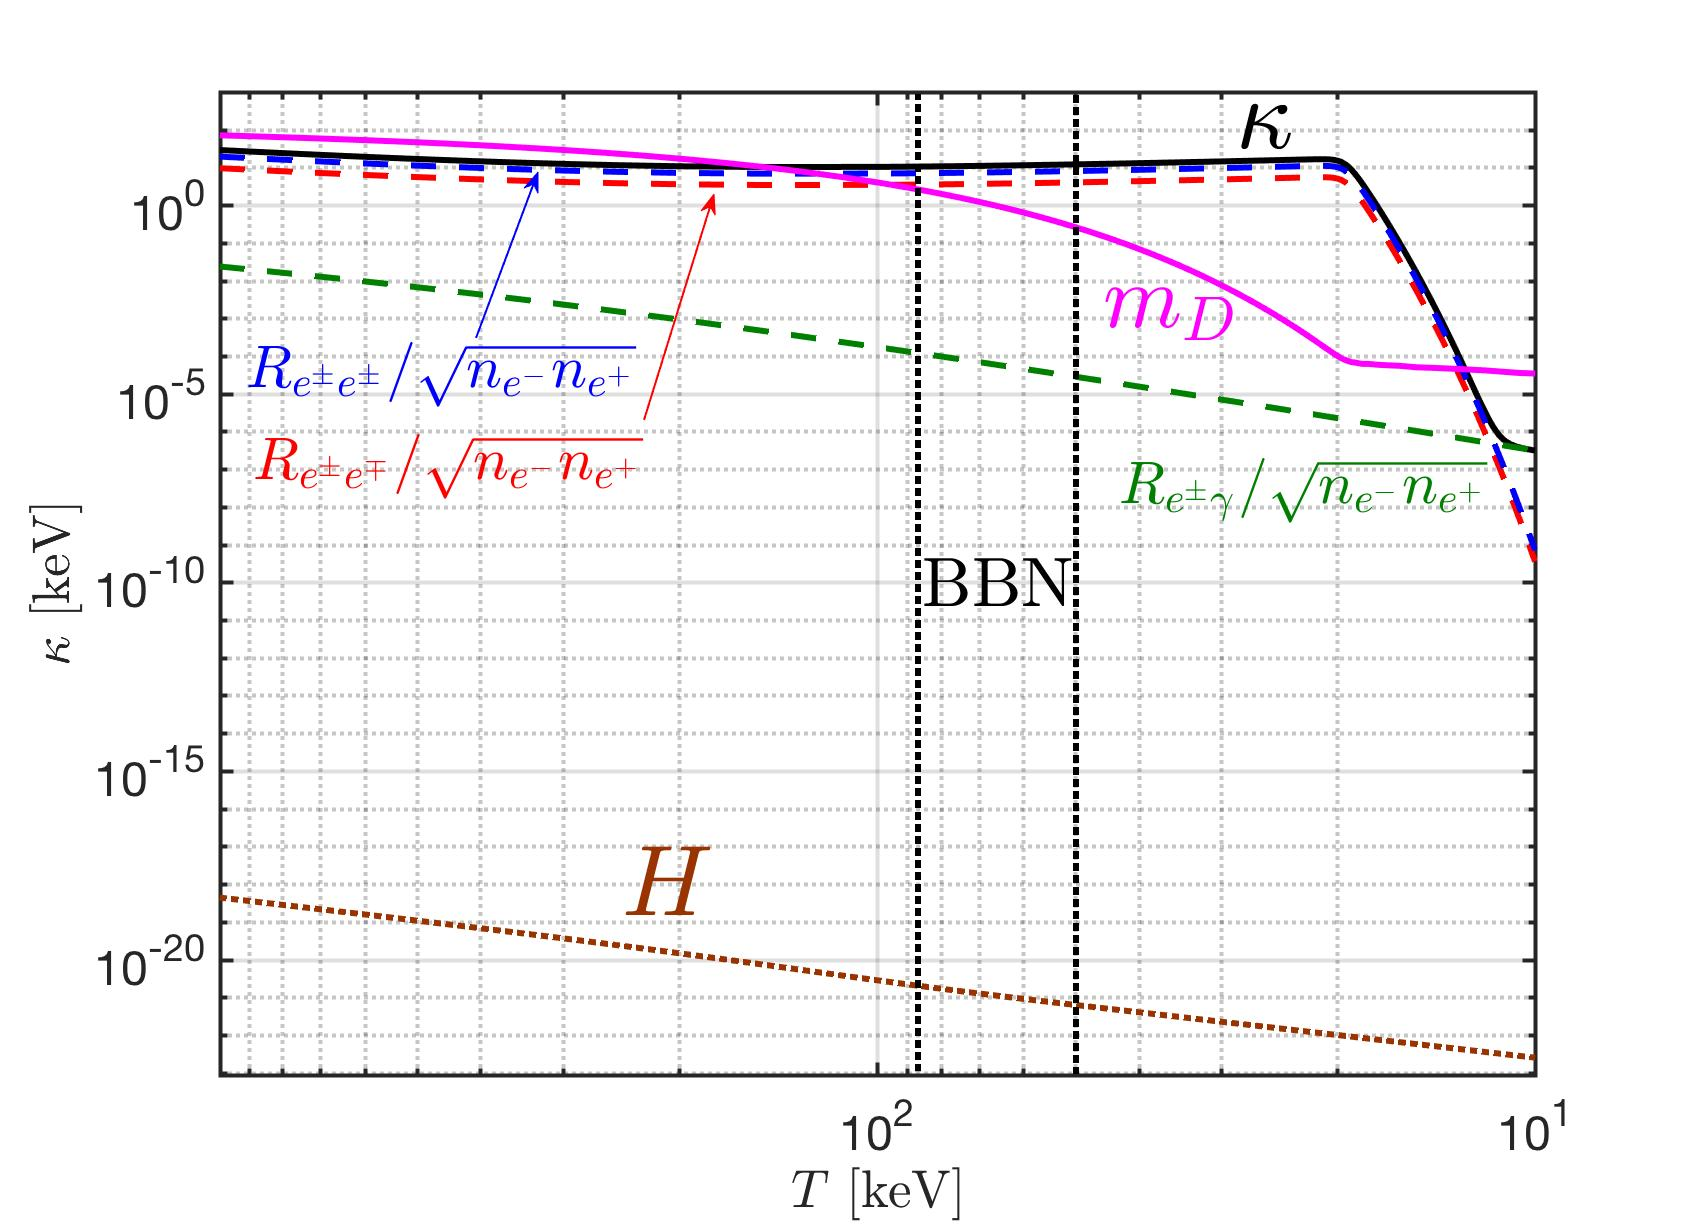
\includegraphics[width=0.8\linewidth]{./plots/May152023Kappa_EPPlasma}}
\caption{The relaxation rate $\kappa$ (black line) as a function of temperature in the nonrelativistic electron-positron plasma, compared to reaction rates for M{\o}ller reaction $e^-+e^-\to e^-+e^-$ (blue dashed line), Bhabha reaction $e^-+e^+\to e^-+e^+$ (red dashed line), and inverse Compton scattering $e^-+\gamma\to e^-+\gamma$ (green dashed line) respectively. The Debye mass $m_D=\omega_{p}\sqrt{m_e/T}$ (purple line) is also shown. \cccite{Grayson:2023flr}. \radapt{Yang:2024ret}}
\label{RelaxationRate:fig}
\end{figure}
%%%%%%%%%%%%%%%%%%%%%%%%


%%%%%%%%%%%%%%%%%%%%%%%%%%%%%%%
\para{Self-consistent damping rate}
In electron-positron plasma, the photon mass\index{photon!plasma mass} $m_\gamma^2$ appears in the transition matrices for M{\o}ller and Bhabha reactions, which is one of important parameters in the calculation of the relaxation rate in $e^\pm$ plasma. When evaluating M{\o}ller and Bhabha scattering, we included as is common practice the temperature-dependent mass of the photon obtained in plasma theory without damping. However, in general, the effective mass of the photon depends at a given temperature on all properties of the QED plasma. 

Considering the linear response theory, the dispersion relation for the photon in nonrelativistic $e^\pm$ plasma is given by~\cite{Formanek:2021blc}
\begin{align}\label{dispersion_damping}
w^2=|k|^2+\frac{w}{w+i\kappa}w_{pl}^2,
\end{align}
where $w_{pl}$ is the plasma frequency and $\kappa$ is the average collision rate of $e^\pm$ plasma. The effective plasma frequency in damped plasma can be solved by considering the case $|k|^2=0$~\cite{Formanek:2021blc}
\begin{align}\label{plasmafrequency_damped}
w_{\pm}=-i\frac{\kappa}{2}\pm\sqrt{w^2_{pl}-\frac{\kappa^2}{4}}.
\end{align}
The result shows that the plasma frequency in damped plasma $w_\pm$ is a function of $\kappa$ which we are computing using the effective plasma photon mass. 

The effective photon mass in damped plasma is also a function of the scattering rate. We have
\begin{align}\label{PhotonMass:self}
m_\gamma=w_\pm(w_{pl},\kappa)=m_\gamma(w_{pl},\kappa),
\end{align}
where the photon mass $m_\gamma=w_+$ for the under-damped plasma $w_{pl}>\kappa/2$, and $m_\gamma=w_-$ for over-damped plasma $w_{pl}<\kappa/2$. \req{PhotonMass:self} shows that computed damping strength $\kappa$ is the dominant scale for collisional plasma and it is also the main parameter determining the photon mass in plasma. 

Substituting the effective photon mass \req{PhotonMass:self} into the definition of the average relaxation rate \req{Kappa}, we obtain a self-consistent equation for damping rate $\kappa$ 
\begin{align}\label{RealaxtionSelf}
\kappa\,\left[\frac{g_e}{2\pi^3}T^3\left(\frac{m_e}{T}\right)^2K_2(m_e/T)\right]=\frac{g_eg_e}{32\pi^4}T\!\! \int_{4m_e^2}^\infty\!\!\!\!ds&
\frac{s(s-4m^2_e)}{\sqrt{s}}K_1(\sqrt{s}/T)
%\times\\&\notag
\bigg[\sigma_{e^\pm e^\pm}(s,w_{pl},\kappa)+\sigma_{e^\pm e^\mp}(s,w_{pl},\kappa)\bigg],
\end{align}
where the cross-sections depend on the parameter $w_{pl}$ and $\kappa$, and the variable $\kappa$ appears on both sides of the equation so we need solve the equation numerically to determine the $\kappa$ value that satisfies this condition.

Depending on the nature of the plasma (overdamped or underdamped plasma), we can establish the photon mass in collision plasma based on two distinct conditions as follows:
\begin{itemize}
\item Case 1. The plasma frequency is larger than the collision rate $w_{pl}>\kappa/2$, we have
\begin{align}
m_\gamma=w_+=-i\frac{\kappa}{2}+\sqrt{w^2_{pl}-\frac{\kappa^2}{4}}.
\end{align}
\item Case 2. The plasma frequency is smaller than the collision rate $w_{pl}<\kappa/2$, we have
\begin{align}\label{PhotonMassPlasma}
m_\gamma=w_-=-i\left(\frac{\kappa}{2}+\sqrt{\frac{\kappa^2}{4}-w^2_{pl}}\right).
\end{align}
\end{itemize}
In \rf{RelaxationRate002:fig} we see that during the BBN epoch $50\leqslant T\leqslant 86$\,keV, the plasma frequency is smaller than the collision rate $w_{pl}<\kappa/2$. In this case, the effective photon mass in collision plasma is given by the overdamped relation \req{PhotonMassPlasma}. This result is valid for $T>20.3$\,keV. For temperature $T<20.3$\,keV, the composition turns into electron and proton plasma, which is beyond our current study because of assumed (for simplicity) equal numbers of electrons and positrons.

%%%%%%%%%%%%%%%%%%%%%%%%%%%%%%%%%
\begin{figure} 
\centerline{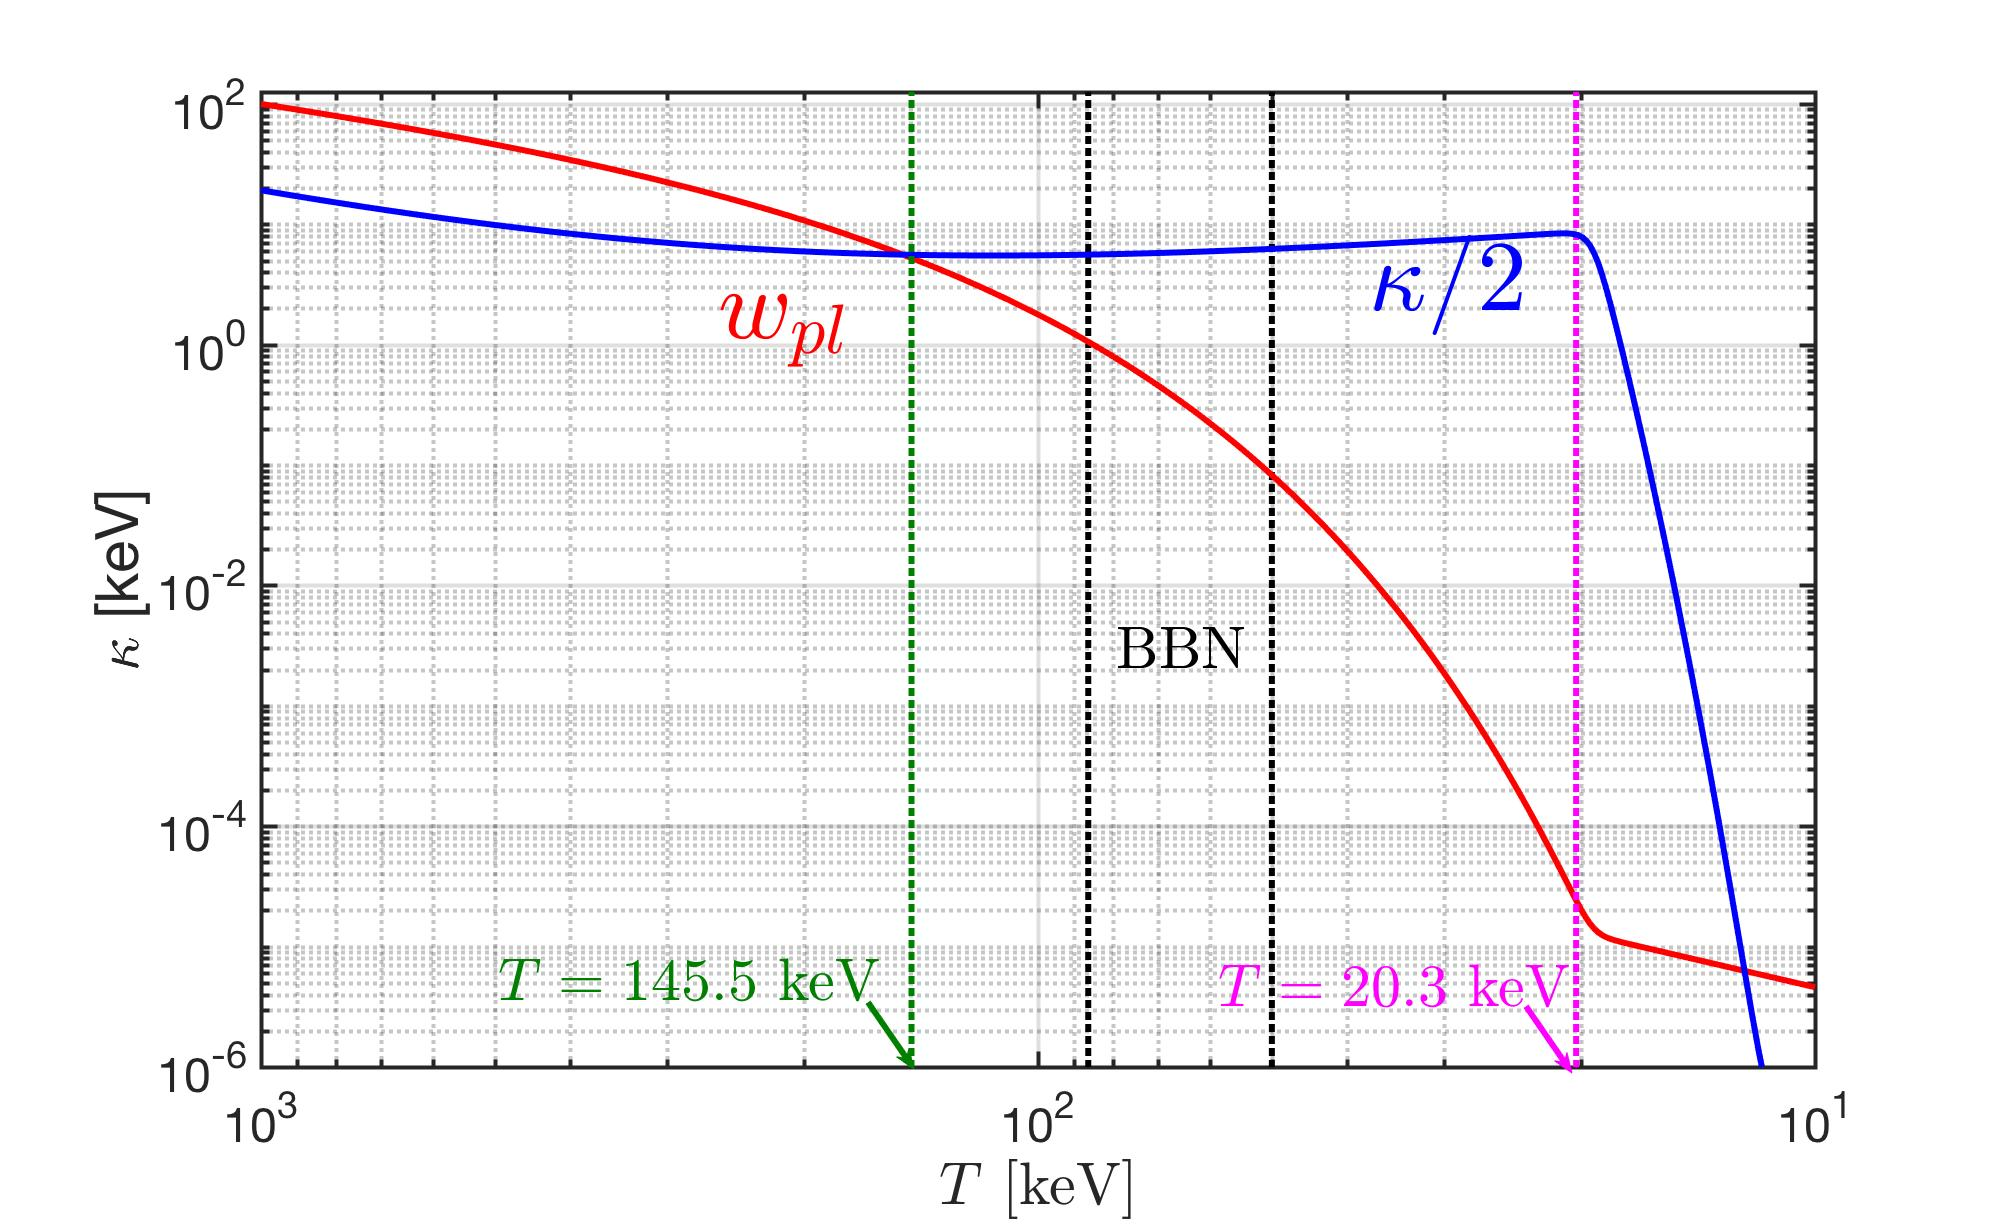
\includegraphics[width=0.8\linewidth]{./plots/KappaElectronPhotonMass_Talk}}
\caption{The relaxation rate $\kappa/2$ (blue line) and plasma frequency $\omega_{pl}$ (red line) as a function of temperature in nonrelativistic electron-positron plasma. Vertical green dashed line indicates the boundary between over- and under-damped plasma at $T<145.5$\,keV which is before the BBN epoch (vertical black lines). Temperature domain of validity is above disappearance of positrons (vertical line at 20.3\,keV). \radapt{Yang:2024ret}}
\label{RelaxationRate002:fig} 
\end{figure}
%%%%%%%%%%%%%%%%%%%%%%%%%%%%%%%%%%%%%%%%%

To calculate the effective cross-sections for M{\o}ller\index{M{\o}ller scattering} and Bhabha\index{Bhabha scattering} scattering we need in the overdamped regime to account for the imaginary photon mass in the calculation of reaction matrix elements. This imaginary part of the photon mass accounts for the decay in sense of propagation range of the massive photon in plasma. We now make a first estimate of the effect of self-consistent real part of the photon mass on the damping rate $\kappa$, we leave the photon decay to a future study.

For BBN\index{Big-Bang!BBN} temperature $50\leqslant T\leqslant 86$\,keV,
we have $w_{pl}<\kappa$ and the effective photon mass can be approximated as
\begin{align}
m^2_\gamma=w_-w_-^\ast&=\left(\frac{\kappa}{2}+\sqrt{\frac{\kappa^2}{4}-w^2_{pl}}\right)^2
=\frac{\kappa^2}{2}\left[\left(1-\frac{2w^2_{pl}}{\kappa^2}\right)+\sqrt{1-\frac{4w^2_{pl}}{\kappa^2}}\right]\notag\\
&=\frac{\kappa^2}{2}\left[\left(1-\frac{2w^2_{pl}}{\kappa^2}\right)+\left(1-\frac{2w^2_{pl}}{\kappa^2}+\cdots\right)\right]\approx\kappa^2\,,
\label{PhotonMassPlasma002}
\end{align}
where we consider the limit $w^2_{pl}/\kappa^2\ll 1$ and effective photon mass is equal to the average collision rate in plasma $m^2_\gamma\approx\kappa$.

Substituting the photon mass $m^2_\gamma=\kappa^2$ for overdamped plasma into the relaxation rate of electron-positron \req{RealaxtionSelf}, and introducing the following dimensionless variables
\begin{align}
x=\sqrt{s}/T,\qquad a=m_\gamma/T=\kappa/T,\qquad b=m_e/T,
\end{align}
the relaxation rate of electron-positron can be written as
\begin{align}\label{Numerical_eq}
&\left[\frac{g_e}{2\pi^2}T^4\left(\frac{m_e}{T}\right)^{\!2}\!K_2(m_e/T)\right]\,\left(\frac{\kappa}{T}\right)\notag\\
&\qquad\qquad\qquad=\frac{g^2_e\alpha^2}{8\pi^3}T^4\!\!\int_{2b}^\infty\!dxK_1(x)\left[\mathcal{F}_{e^\pm e^\pm}(x,\kappa/T)+\mathcal{F}_{e^\pm e^\mp}(x,\kappa/T)\right],
\end{align}
where the functions $\mathcal{F}_{e^\pm e^\pm}$ and $\mathcal{F}_{e^\pm e^\mp}$ are given by
\begin{align}
\mathcal{F}_{e^\pm e^\pm}(x,a=\kappa/T)&=\left\{2\left[3a^2+4b^2+\frac{4(b^4-a^4)}{x^2-4b^2+2a^2}\right]\ln\left(\frac{a^2}{x^2-4b^2+a^2}\right)\right.\notag\\
&\left.+\frac{(x^2-4b^2)(8b^4+2a^4+3a^2x^2+2x^4-4b^2(2x^2+a^2))}{a^2(x^2-4b^2+a^2)}\right\}
\end{align}
and 
\begin{align}
\mathcal{F}_{e^\pm e^\mp}(x,a=\kappa/T)&=\left\{\frac{2x^2(a^2+x^2)-4b^4}{x^2-a^2}\ln\left(\frac{a^2}{x^2-4b^2+a^2}\right)\right.\notag\\
&+\frac{(x^2-4b^2)(3x^2+4b^2+2a^2)}{(x^2-a^2)}+\frac{x^6-12b^4x^2-16b^6}{3(x^2-a^2)^2}\notag\\
&\left.+\frac{(x^2-4b^2)(8b^4+2a^4+3a^2x^2+2x^4-4b^2(2x^2+a^2))}{a^2(x^2-4b^2+a^2)}\!\right\}.
\end{align}

We solve \req{Numerical_eq} numerically. In \rf{KappaSol:fig}, we plot the resultant relaxation rate $\kappa$ that satisfies \req{Numerical_eq} as a function of temperature $50\,\mathrm{keV} \leqslant T\leqslant 86$\,keV. The result shows that in the the BBN temperature range, the overdamping is considerably reduced: We remember that we started with $w_{pl}<\kappa$, and the effective photon mass $m^2_\gamma=\kappa^2$. Now we obtain a relaxation rate $\kappa=1.832\sim 0.350$\,keV during BBN epoch, which is smaller than the relaxation rate without damping effect on the photon mass, compare \rf{RelaxationRate:fig}, where the relaxation rate $\kappa=10\sim12$\,keV during the BBN epoch is shown.\index{plasma damping}

%%%%%%%%%%%%%%%%%%%%%%%%%%%%%%%%%%%%%%%%%%%%%%
\begin{figure} 
\centerline{
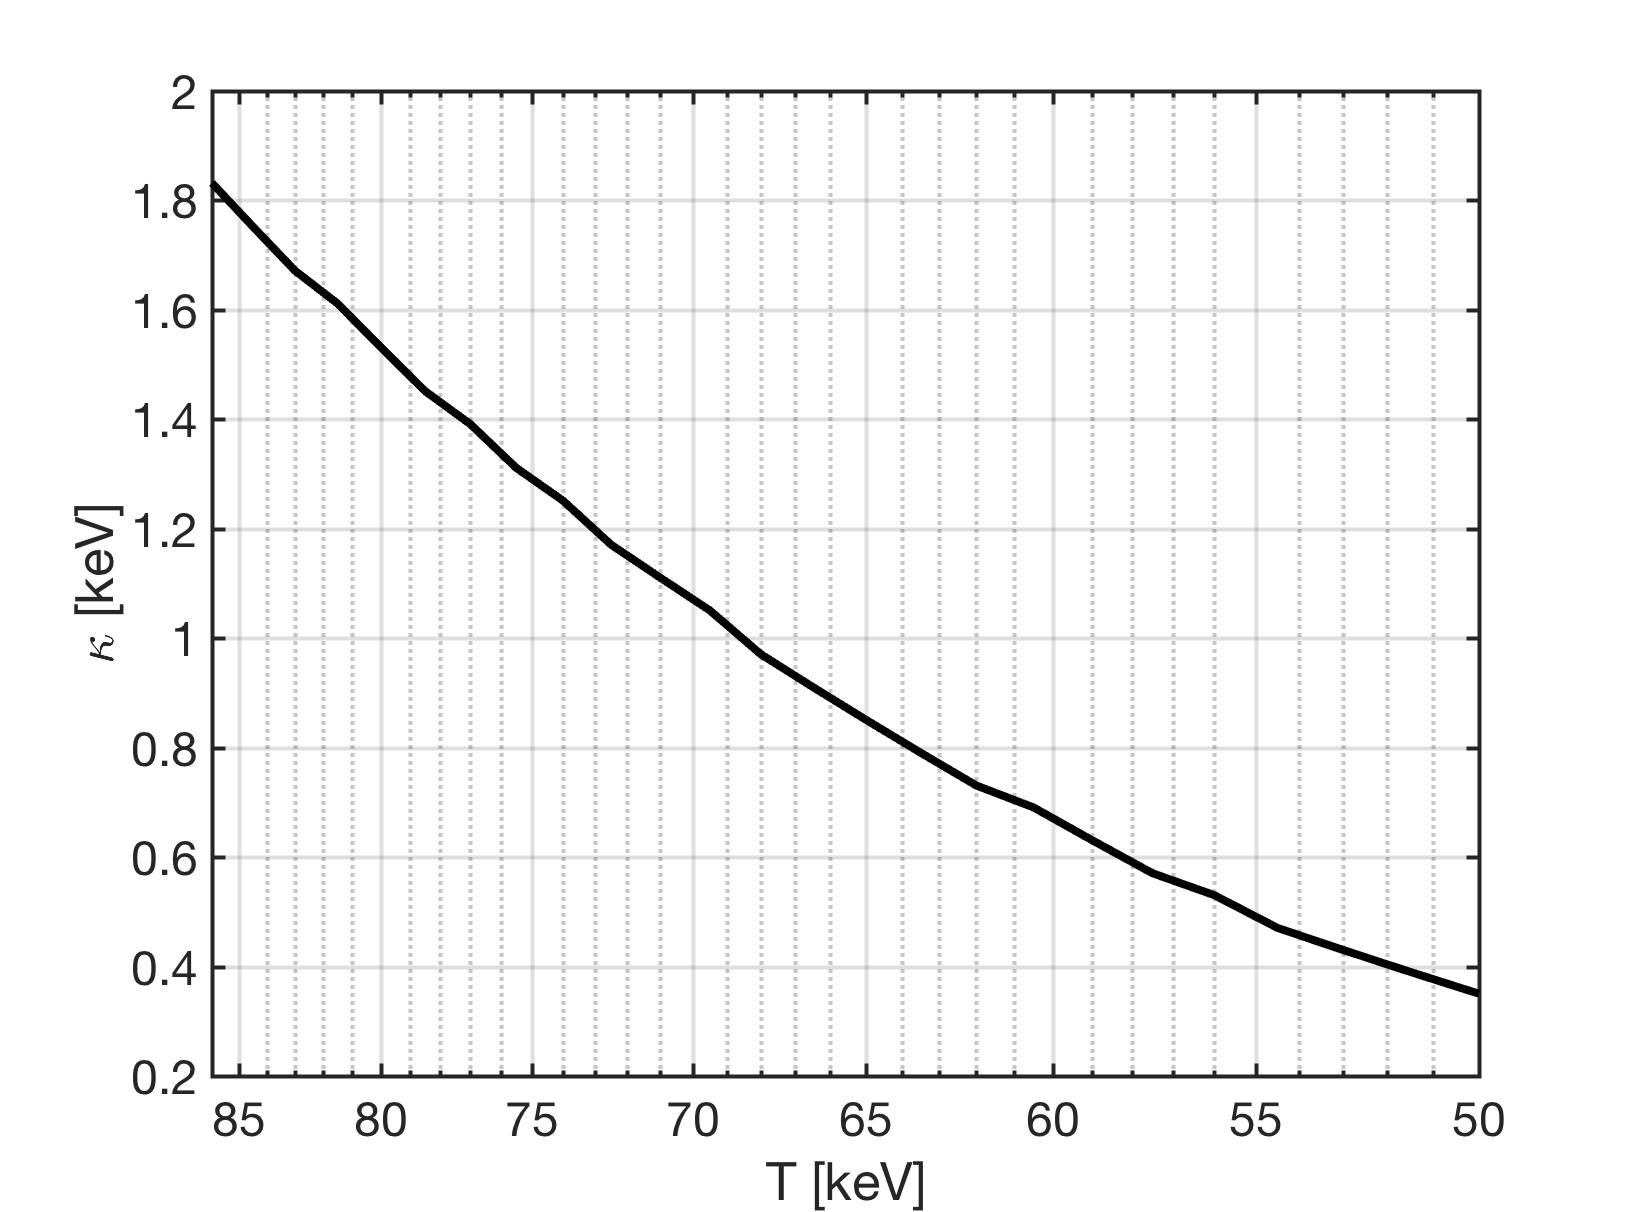
\includegraphics[width=0.8\linewidth]{./plots/OverdampingKappa.jpg}}
\caption{The relaxation rate $\kappa$ that satisfies \req{Numerical_eq} self-consistently as a function of temperature $50\leqslant T\leqslant 86$\,keV. The minor fluctuations are due to limited numerical precision. \radapt{Yang:2024ret}}
\label{KappaSol:fig} 
\end{figure}
%%%%%%%%%%%%%%%%%%%%%%%%%%%%%%%%%%%%%%%%%%

This first estimate of self-consistent plasma damping shows high sensitivity, demonstrating the need for a full self-consistent evaluation of damping rate in plasma within the context of a well-defined, self-consistent approach, where both damping and photon properties in plasma are determined in a mutually consistent manner, a project which is well ahead of the current state of the art and which is well beyond the scope of this report. 

